\documentclass{article}%
\usepackage[T1]{fontenc}%
\usepackage[utf8]{inputenc}%
\usepackage{lmodern}%
\usepackage{textcomp}%
\usepackage{lastpage}%
\usepackage[head=40pt,margin=0.5in,bottom=0.6in]{geometry}%
\usepackage{graphicx}%
%
\title{\textbf{Jueza militar que huyó a Colombia pidió perdón a Gilber Caro}}%
\author{El Nacional Web}%
\date{02/10/2018}%
%
\begin{document}%
\normalsize%
\maketitle%
\textbf{URL: }%
http://www.el{-}nacional.com/noticias/politica/jueza{-}militar{-}que{-}huyo{-}colombia{-}pidio{-}perdon{-}gilber{-}caro\_254099\newline%
%
\textbf{Periodico: }%
EN, %
ID: %
254099, %
Seccion: %
Política\newline%
%
\textbf{Palabras Claves: }%
Política\newline%
%
\textbf{Derecho: }%
1.2, %
Otros Derechos: %
1.10, %
Sub Derechos: %
1.2.2, 1.10.1\newline%
%
\textbf{EP: }%
NO\newline%
\newline%
%
\textbf{\textit{Luz Mariela Acevedo se encuentra actualmente en Colombia luego de que huyera de Venezuela}}%
\newline%
\newline%
%
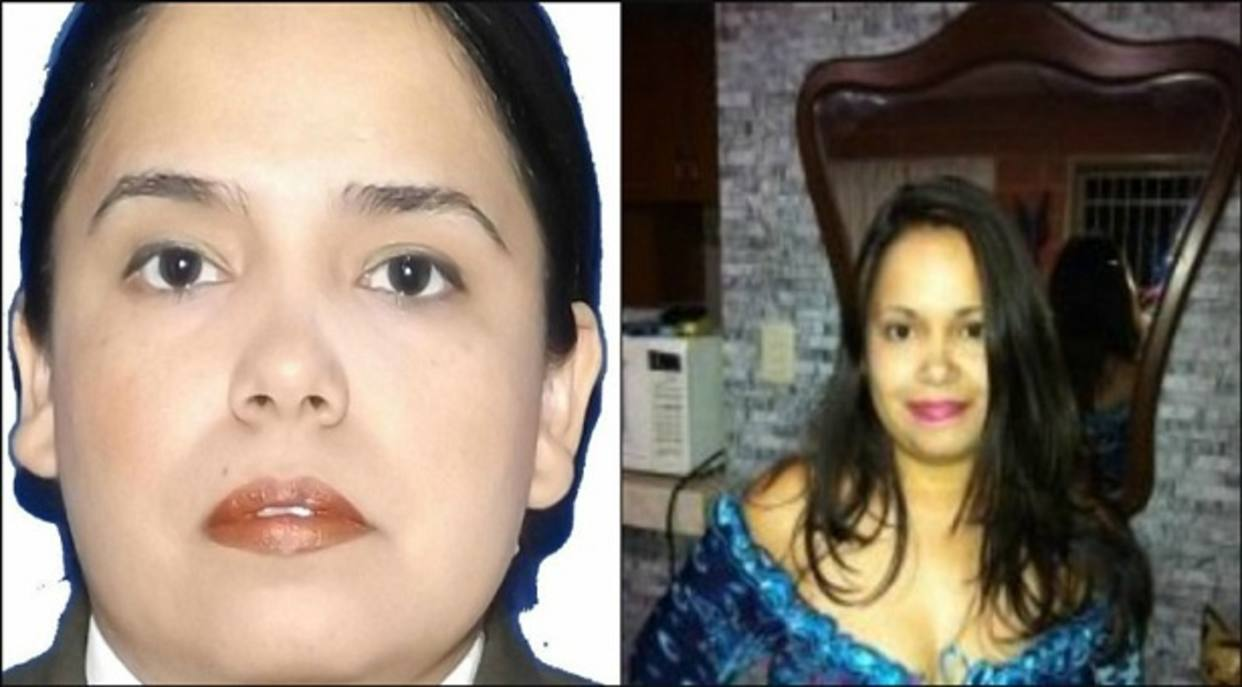
\includegraphics[width=300px]{59.jpg}%
\newline%
%
Luz Mariela Acevedo, capitana y jueza militar encargada de procesar civiles ante la justicia militar, reveló este martes que ofreció disculpas a Gilber Caro, diputado a la Asamblea Nacional, por haber procesado su caso en un tribunal militar.%
\newline%
%
“Yo realmente pido perdón a todos aquellos que les cause daño en alguna oportunidad. Yo le pedí perdón a Gilber~Caro”, indicó Acevedo durante una entrevista en~EvTV Miami.%
\newline%
%
La jueza indicó además que si bien en el seno de la Fuerza Armada hay funcionarios que están en desacuerdo con el gobierno de Nicolás Maduro, hay mucho temor a actuar.%
\newline%
%
“Sé que dentro de la Fuerza Armada hay mucha gente que aunque no está de acuerdo, pero tienen miedo”, aseveró.%
\newline%
%
Los señalamientos de Acevedo ocurren luego de que huyera a Colombia buscando refugio alegando la situación social y económica que vive Venezuela.%
\newline%
%
\end{document}